\normaltrue \difficilefalse \tdifficilefalse
\correctionfalse

%\UPSTIidClasse{11} % 11 sup, 12 spé
%\newcommand{\UPSTIidClasse}{12}
% ATS 2019
\exer{Vérin double effets $\star$ \label{SYS:01:A3:05:1100}}
\setcounter{question}{0}\marginnote{\xpComp{SYS}{01}}
\index{Compétence A3-05}
\index{Compétence SYS-01}
\index{Distributeur}
\index{Vérin}
\ifcorrection
\else
\marginnote{\textbf{Pas de corrigé pour cet exercice.}}
\fi


Un vérin double effet est commandé par un distributeur 4/2 (4 orifices, 2 positions) bi-stable.



\begin{marginfigure}
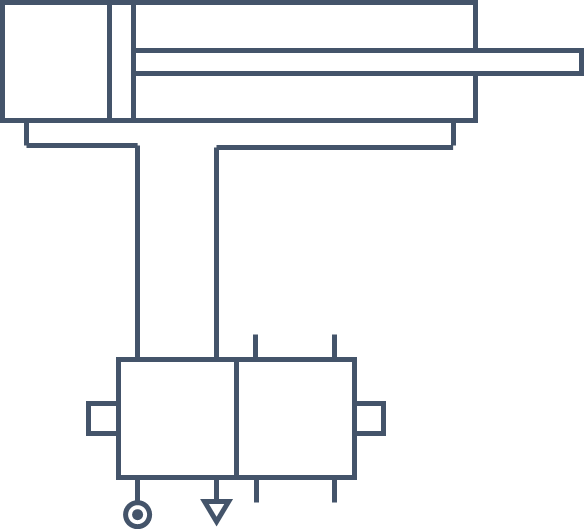
\includegraphics[width=\linewidth]{1100_fig_01}
%\textit{}
\end{marginfigure}

\question{Compléter le câblage du distributeur.}

\question{Dans la position actuelle, indiquer par des flèches le sens de déplacement du vérin. Indiquer en rouge les tuyaux et chambre hautes pressions. Indiquer en bleu les tuyaux et chambre basses pressions.}

\question{On souhaite ralentir le déplacement du vérin lorsqu'il sort de la chambre. Positionner le limiteur de débit en conséquence.}

\begin{marginfigure}
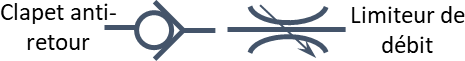
\includegraphics[width=\linewidth]{1100_fig_02}
%\textit{}
\end{marginfigure}


\question{Ajouter un clapet anti-retour pour éviter la limitation du débit lorsque le vérin se rétracte.}


Au démarrage du véhicule, la valve de décharge du module (b) est fermée. Le distributeur à effet proportionnel(e) est en position médiane, les vérins sont donc immobiles. La commande des vérins est initialement bloquée par une temporisation.

\question{En considérant les conditions initiales évoquées, expliquer, en commençant à l’instant de démarrage de la pompe, le comportement du circuit hydraulique en précisant clairement les différentes phases de fonctionnement. Quel est l’utilité de la temporisation ? On souhaite remplacer cette temporisation par un capteur. Préciser la grandeur qu’il devra mesurer. Donner un avantage et un inconvénient du remplacement de la temporisation par ce capteur.}
\ifprof
\begin{corrige}
Démarrage de la pompe et montée en pression du circuit avec remplissage de l’accumulateur (c).

À la fin de la temporisation le distributeur peut être commandé et ainsi alimenter les vérins.

Si la pression augmente trop, alors le limiteur de pression (d) renvoie une partie du fluide vers le
réservoir et si c’est insuffisant alors (b) permet une décharge du circuit (ouverture vers le réservoir
jusqu’à atteindre ne niveau bas réglé).

La temporisation permet d’attendre qu’un niveau de pression suffisant dans le circuit soit atteint.

Pour remplacer la temporisation on peut mesurer la pression dans le circuit ou plus simplement détecter
le niveau de pression satisfaisant pour le fonctionnement à l’aide d’un pressostat.

La solution utilisant un capteur de pression est plus sûre que la temporisation qui pourrait autoriser la
commande du distributeur alors que la pression dans le circuit est encore insuffisante.

(UPSTI). 
\end{corrige}
\else
\fi


\ifprof
\else
\marginnote{Corrigé  voir \ref{SYS:01:A3:05:1100}.}
\fi